\documentclass{standalone}
\usepackage{pgfplots}
\usepackage{xcolor}
\usepgfplotslibrary{statistics}
\pgfplotsset{compat=1.17}

% Auburn colors
\definecolor{auburnorange}{RGB}{232, 119, 34}
\definecolor{auburnblue}{RGB}{12, 35, 64}
\definecolor{lightbluegray}{RGB}{220,230,240}

\begin{document}
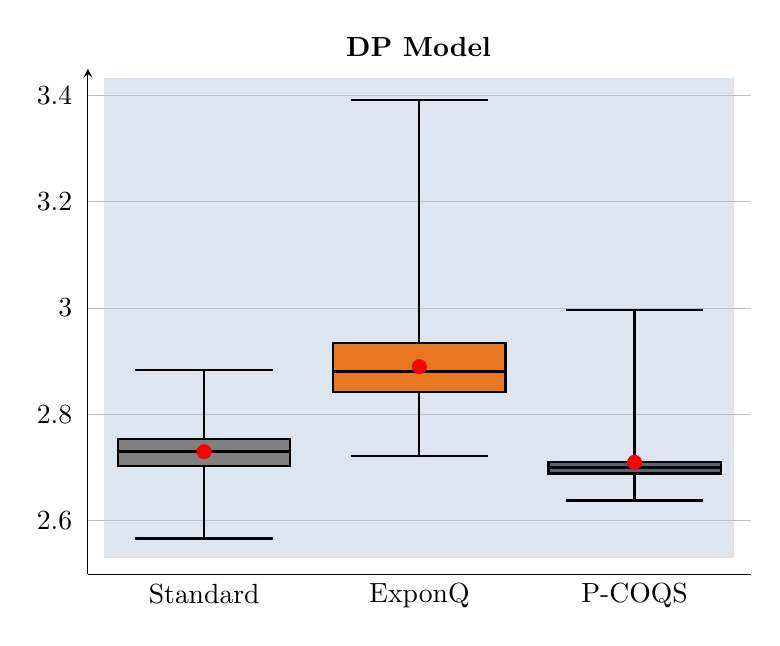
\begin{tikzpicture}

% Background for DP models
\fill [lightbluegray] (0.2,0.2) rectangle (8.2,6.3);

\begin{axis}[
    boxplot/draw direction=y,
    %ylabel={Avg. Prediction Set Size},
    xtick={1,2,3},
    xticklabels={
        {Standard},
        {ExponQ},
        {P-COQS}
    },
    x tick label style={align=center},
    ymin=2.5, ymax=3.45,
    width=10cm,
    height=8cm,
    ymajorgrids,
    axis x line*=bottom,
    axis line style={-},
    axis y line=left,
    tick style={draw=none},
    enlarge x limits=0.05,
    boxplot/every box/.style={draw=black, thick, solid},
    boxplot/every whisker/.style={black},
    boxplot/every median/.style={black, very thick},
]

% Standard (DP)
\addplot+[
    draw=black, solid, thick,
    fill=gray,
    boxplot prepared={
        lower whisker=2.5668,
        lower quartile=2.7024,
        median=2.7302,
        upper quartile=2.7546,
        upper whisker=2.8838
    },
] coordinates {};

% ExponQ (DP)
\addplot+[
    draw=black, solid, thick,
    fill=auburnorange,
    boxplot prepared={
        lower whisker=2.7222,
        lower quartile=2.8418,
        median=2.8812,
        upper quartile=2.9342,
        upper whisker=3.3906
    },
] coordinates {};

% P-COQS (DP)
\addplot+[
    draw=black, solid, thick,
    fill=auburnblue!70,
    boxplot prepared={
        lower whisker=2.6384,
        lower quartile=2.6892,
        median=2.6998,
        upper quartile=2.7106,
        upper whisker=2.9958
    },
] coordinates {};

% Red mean dots
\addplot[
    only marks,
    mark=*,
    mark size=2.5pt,
    red
] coordinates {
    (1, 2.73)
    (2, 2.89)
    (3, 2.71)
};

\end{axis}

\node at (4.2,6.7) {\textbf{DP Model}};

\end{tikzpicture}
\end{document}
